\newpage
\section{Experiment 1: Low Pass Filter}

\subsection{Objective}
To determine the input/output characteristics of a low pass filter and calculate its cut-off frequency.

\subsection{Instruments}
\begin{itemize}
\item Oscilloscope
\item Function generator
\item EC2 MVM6 box
\end{itemize}

\subsection{Theory}
\subsubsection*{Introduction}

Low-pass filters play a crucial role in signal processing, allowing the passage of low-frequency signals while attenuating higher frequencies. This experiment aims to analyze the input/output characteristics of a low-pass filter and determine its cut-off frequency (\(f_c\)), which signifies the point at which the filter starts attenuating the input signal significantly.

\subsubsection*{Low-Pass Filter Characteristics}

The transfer function of a first-order low-pass filter is given by:

\[
H(f) = \frac{1}{1 + j\left(\frac{f}{f_c}\right)}
\]

where \(f\) is the input frequency, \(f_c\) is the cut-off frequency, and \(j\) is the imaginary unit.

\subsubsection*{Cut-Off Frequency}

The cut-off frequency is a critical parameter in understanding low-pass filter behavior. It is related to the time constant (\(\tau\)) of the filter by the equation:

\[
f_c = \frac{1}{2\pi\tau}
\]

A low-pass filter can be implemented using an operational amplifier (op-amp) as the active element and resistors and capacitors as passive elements. The generic filter diagram is shown in Figure \ref{fig:A15.1}, where $Z1-Z5$ indicate generic impedances. The input-output formula for the general diagram is given by:

\begin{equation}
    \frac{Vo}{Vin} = \frac{Z2 \cdot Z4 \cdot Z5}{Z1 \cdot Z3 \cdot Z5 + Z1 \cdot Z2 \cdot Z5 + Z1 \cdot Z2 \cdot Z3 + Z2 \cdot Z3 \cdot Z5 - Z2 \cdot Z1 \cdot Z4}
\end{equation}

This relation assumes ideal conditions such as infinite input impedance and infinite amplification of the operational amplifier, leading to a virtual ground.

% \begin{figure[H]
%     \centering
%     \includegraphics[scale=0.6]{fig_A15.1.png}
%     \caption{Generic low-pass filter diagram.}
%     \label{fig:A15.1}
% \end{figure}

For a specific low-pass filter with resistors ($Z1$, $Z3$, and $Z5$) and capacitors ($Z2$ and $Z4$), the input-output formula becomes:

\begin{equation}
    \frac{Vo}{Vin} = \frac{R2 \cdot R3 \cdot C1 \cdot C2}{R3 + R2 \cdot (1 + j \omega R1 \cdot C1)}
\end{equation}

where $\omega$ is the angular frequency of the input signal.

The cut-off frequency $F_c$ is determined by the values of the passive components:

\begin{equation}
    F_c = \frac{1}{2 \pi R1 \cdot R2 \cdot C1 \cdot C2}
\end{equation}

The gain $G_0$ of the filter at DC (frequency $f = 0$ Hz) is given by:

\begin{equation}
    G_0 = -\frac{R3}{R1}
\end{equation}
\subsubsection*{Experiment Setup}

The experiment utilizes an oscilloscope, function generator, and the EC2 MVM6 box. The function generator provides the input signal, and the oscilloscope measures the output signal. The EC2 MVM6 box contains the low-pass filter circuit under investigation.

\subsubsection*{Procedure}

\begin{enumerate}
    \item Connect the function generator output to the input of the low-pass filter circuit.
    \item Connect the output of the low-pass filter circuit to the input channel of the oscilloscope.
    \item Set the function generator to produce a sine wave with varying frequencies.
    \item Measure and record the amplitude of the output signal at different input frequencies.
\end{enumerate}


\subsubsection*{Expected Results}

The input/output characteristics of the low-pass filter are expected to show a gradual attenuation of the output amplitude as the input frequency increases. The cut-off frequency can be determined by analyzing the point at which the attenuation becomes significant.

\subsubsection*{Significance}

Understanding low-pass filter behavior is crucial in applications such as audio signal processing, communication systems, and control systems. Determining the cut-off frequency allows for the design of filters tailored to specific frequency ranges, optimizing electronic system performance.


\subsection{Results}
% Present the results of the second experiment.
\subsection*{Q1: What is the approximate amplification of the filter at 10 Hz?}

\begin{enumerate}
    \item 1
    \item 9
    \item 15
    \item 50
    \item Infinite
\end{enumerate}

\subsection*{Q2: What is the main reason for this amplification value?}
\begin{itemize}
    \item 1 the value of $R22$
    \item 2 the value of $C10$
    \item 3 the value of $R23$
    \item 4 the value of the ratio $\frac{R23}{R20}$
    \item 5 the value of the product $R22 \cdot C10$
\end{itemize}


\begin{table}[H]
    \centering
    \begin{tabular}{|c|c|}
        \hline
        \textbf{Input Frequency (Hz)} & \textbf{Output Amplitude (Vpp)} \\
        \hline
        10 & 9.1 \\
        20 & 9.2 \\
        40 & 8.8 \\
        60 & 8.7 \\
        80 & 8.6 \\
        100 & 8.0 \\
        150 & 6.3 \\
        200 & 4.5 \\
        500 & 2.5 \\
        \hline
    \end{tabular}
    \caption{Input frequency and output amplitude measurements.}
    \label{table:A15.1}
\end{table}

Plot all the values obtained into figure A15.4 and draw the
input/output characteristic of the filter

From this graph calculate the cut-off frequency of the filter, defined
as the frequency at which the amplification drops to 0.707 times the
maximum. 

\begin{figure}[H]
    \centering
    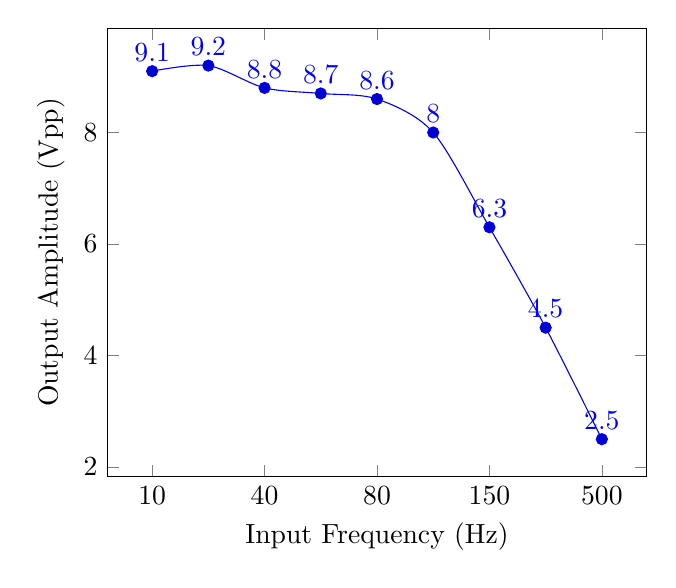
\begin{tikzpicture}
        \begin{axis}[
            xlabel={Input Frequency (Hz)},
            ylabel={Output Amplitude (Vpp)},
            legend style={at={(0.5,-0.15)}, anchor=north},
            symbolic x coords={10, 20, 40, 60, 80, 100, 150, 200, 500},
            nodes near coords,
            nodes near coords align={vertical},
            smooth,
            mark=square,
        ]
        \addplot table {
            InputFrequency OutputAmplitude
            10 9.1
            20 9.2
            40 8.8
            60 8.7
            80 8.6
            100 8.0
            150 6.3
            200 4.5
            500 2.5
        };
        \end{axis}
    \end{tikzpicture}
    \caption{Input frequency vs. output amplitude (A15.4)}
    \label{fig:A15.4_graph}
\end{figure}

\subsection*{Turn switch S22 ``ON''}
\begin{itemize}
    \item Now measure the cut-off frequency of the filter again.
\end{itemize}

\subsubsection*{Q3: What do you notice?}
\begin{itemize}
    \item[\textendash] 1 the cut-off frequency is increased
    \item[\textendash] 2 the cut-off frequency is decreased
    \item[\textendash] 3 the output voltage is constant
    \item[\textendash] 4 the output voltage is a square wave
    \item[\textendash] 5 the output voltage is a triangular wave
\end{itemize}

\subsubsection*{Q4: What is the cause of this?}
\begin{itemize}
    \item[\textendash] 1 the output is short-circuited
    \item[\textendash] 2 the inputs are short-circuited
    \item[\textendash] 3 the capacitor C10 has increased
    \item[\textendash] 4 the capacitor C10 has decreased
    \item[\textendash] 5 the amplifier has positive feedback
\end{itemize}
\subsection{Conclusion}
% Summarize the key findings of both experiments and their overall implications.

\subsection{References}
% List your references using BibTeX or manually.